\documentclass[12pt]{report}

\textheight 22cm
\textwidth 15.5cm
\oddsidemargin 0pt\evensidemargin 0pt
%\oddsidemargin 14pt\evensidemargin 0pt
%\topmargin -40pt
\topmargin-30pt
%\bottommargin0pt
\def\baselinestretch{1.1}
%\addtolength{\parskip}{1ex}
\jot=.5ex
%\parskip = 0.02in


\setlength\arraycolsep{2pt}


\usepackage{amssymb}
\usepackage{amsmath,bm}
\usepackage{amssymb}
\usepackage{graphicx}
\usepackage{amsfonts}         
\usepackage{fancybox}   

%\usepackage[numbers]{natbib}

\usepackage{enumitem}

\usepackage{slashed}




\usepackage[usenames,dvipsnames]{xcolor}%http://en.wikibooks.org/wiki/LaTeX/Colors

\definecolor{darkgreen}{rgb}{0,0.4,0}
\definecolor{darkred}{rgb}{0.4,0,0}
\definecolor{darkblue}{rgb}{0,0,0.4}
\definecolor{lightblue}{rgb}{.6,.6,0.9}
\newcommand{\cobl}{\color{darkblue}}

\newcommand{\cor}{\color{red}}
\newcommand{\cog}{\color{darkgreen}}
\newcommand{\cob}{\color{black}}

\definecolor{uglybrown}{rgb}{0.8,  0.7,  0.5}


\def\nd{{ \vphantom{\dagger}}}

\def\dd{\text{d}}
\def\dbar{{\mathchar'26\mkern-12mu \dd}} 

\def\ii{{\bf i}}
\def\Ione{\mathbb{I}}
\def\UU{{\bf U}}
\def\HH{{\bf H}}
\def\pp{{\bf p}}
\def\aa{{\bf a}}
\def\qq{{\bf q}}
\def\eps{\epsilon}
\def\half{{1\over 2}}
\def\Tr{{{\rm Tr~ }}}
\def\tr{{\rm tr}}
\def\Re{{\rm Re\hskip0.1em}}
\def\Im{{\rm Im\hskip0.1em}}
\def\ppi{\boldsymbol{\pi}}
\def\pphi{\boldsymbol{\phi}}
%\def\pphi{\phi}
\def\grad{\vec \nabla}
\def\vB{\vec B}
\def\vE{\vec E}
\def\vA{\vec A}
\def\vAA{ \vec{\bf A}}
\def\vEE{{{\vec {\bf E}}}}
\def\vBB{{\vec {\bf B}}}
\def\CO{{\cal O}}
\def\CL{{\cal L}}
\def\IZ{\mathbb{Z}}
\def\CN{{\cal N}}

\def\IR{\mathbb{R}}
\def\CD{{\cal D}}


\def\ie{{\it i.e.}}
\def\eg{{\it e.g.}}

\def\bra#1{\left\langle#1\right|}
\def\ket#1{\left|#1\right\rangle}
\def\bbra#1{{\langle\langle}#1|}
\def\kket#1{|#1\rangle\rangle}
\def\vev#1{\left\langle{#1}\right\rangle}

\def\ketbra#1#2{ | #1 \rangle\hskip-2pt\langle #2|}



\def\be{\begin{equation}}
\def\ee{\end{equation}}
\def\({\left(}
\def\){\right)}


\usepackage{tikz}
\usetikzlibrary{decorations.markings}
\usetikzlibrary{arrows,decorations.pathmorphing,backgrounds,positioning,fit,petri,automata,shadows,calendar,mindmap, graphs}

% from flip tanedo.
% Based on:
% http://www.texample.net/tikz/examples/feynman-diagram/

\tikzset{
	% >=stealth', %% more traditional arrows, I don't like them
    vector/.style={decorate, decoration={snake}, draw},
    fermion/.style={postaction={decorate},
        decoration={markings,mark=at position .55 with {\arrow{>}}}},
    fermionbar/.style={draw, postaction={decorate},
        decoration={markings,mark=at position .55 with {\arrow{<}}}},
    fermionnoarrow/.style={},
    gluon/.style={decorate,
        decoration={coil,amplitude=4pt, segment length=5pt}},
    scalar/.style={dashed, postaction={decorate},
        decoration={markings,mark=at position .55 with {\arrow{>}}}},
    scalarbar/.style={dashed, postaction={decorate},
        decoration={markings,mark=at position .55 with {\arrow{<}}}},
    scalarnoarrow/.style={dashed,draw},
%
%%% 	Special vectors (when you need to fine-tune wiggles)
%	provector/.style={decorate, decoration={snake,amplitude=2.5pt}, draw},
%	antivector/.style={decorate, decoration={snake,amplitude=-2.5pt}, draw},
%	    electron/.style={draw=black, postaction={decorate},
%        decoration={markings,mark=at position .55 with {\arrow[draw=black]{>}}}},
%	bigvector/.style={decorate, decoration={snake,amplitude=4pt}, draw},
	vectorscalar/.style={loosely dotted,draw=black, postaction={decorate}},
}




\newcommand{\bea}{\begin{eqnarray}}
\newcommand{\eea}{\end{eqnarray}}


\def\parfig#1#2{
\parbox{#1\textwidth}
{\includegraphics[width=#1\textwidth]{#2}}
}



%%from  Rudro Rana Biswas
\usepackage[pagebackref,  % this puts links to the page numbers where refs appear
%pdftex, 
bookmarks={false}, pdfauthor={John McGreevy}, pdftitle={Yay, physics!}]{hyperref}
\hypersetup{colorlinks=true, 
linkcolor=BrickRed, 
citecolor=Violet, 
filecolor=OliveGreen, 
urlcolor=RoyalBlue, 
filebordercolor={.8 .8 1}, 
urlbordercolor={.8 .8 0}}%http://en.wikibooks.org/wiki/LaTeX/Hyperlinks


%\usepackage{mathtools} % for inclusion arrow \xhookrightarrow{}


\renewcommand{\theequation}{\arabic{equation}}
\newif{\ifeq}           % defines a new condition @eq tested by the conditional \ifeq
\eqtrue                 % if uncommented, declares @eq to be true
\eqfalse              % if uncommented, declares @eq to be false
%                                %
%                                % to use this, wrap text with the conditional, eg:
%                                %
%                                % \ifeq
%                                % SHOW THIS IFF \eqtrue HAS BEEN DECLARED
%                                % \fi
%
\def\answer#1
{
\ifeq
\textcolor{darkblue}{#1}
\fi
}


\begin{document}
\begin{center}

University of California at San Diego -- 
Department of Physics --
Prof.~John McGreevy

{\Large\bf  Physics 215B QFT Winter 2025}\\
{\Large\bf Assignment 5 \answer{--~~~ Solutions} }
\end{center}


\noindent
%Posted September 17, 2015 
\hfill {\bf Due  11:59pm Tuesday, February 11, 2025}




\bigskip
\hrule
\begin{enumerate}

\item {\bf Brain-warmer.}
%\begin{enumerate}
%\item 
%Show that we did the right thing in the numerator of the electron self-energy: 
%use the Clifford algebra to show that 
%$$  \gamma^\mu \( x \slashed{p} + m_0 \) \gamma_\mu = - 2  x \slashed{p}  + 4 m_0 . $$

%\item 
Prove the Gordon identities
$$ \bar u_2  \(q^\nu \sigma_{\mu\nu}   \) u_1 
= \ii \bar u_2  \( (p_1 + p_2)_\mu - (m_1 + m_2) \gamma_\mu \) u_1 
$$ 
and
$$ \bar u_2  \( (p_1+p_2)^\nu  \sigma_{\mu\nu}   \) u_1 
= \ii \bar u_2  \( {\cob(p_2 - p_1)}_\mu - {\cob (m_2 - m_{1})} \gamma_\mu \) u_1 
$$ 
where $q  \equiv {\cob p_2 - p_1} $ and $ \slashed{p}_1 u_1 = m_1 u_1, \bar u_2 \slashed{p}_2 = m_2 \bar u_2$,
using the definitions and the Clifford algebra.
%\end{enumerate}





\item {\bf Tadpole diagrams.}

\begin{enumerate}

\item{}
Why don't we worry about the following diagram 
\vspace{1em}
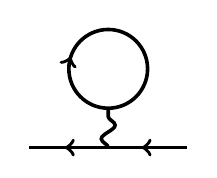
\begin{tikzpicture}[line width=1.3 pt, scale=1]
	\draw[fermion] (0:1)--(0,0);
	% \node at (-140:1.2) {$e$};
	% \node at (140:1.2) {$e$};
	% \node at (.5,.3) {$\gamma$};	
	\draw[fermion] (1.5,1) arc (360:0:.5);
%	\draw[scalarnoarrow] (2,0) arc (0:-180:.5);
	\draw[vector] (1,0) --(1,.5);
	\draw[fermionbar] (1,0) --(2,0);
	% \node at (2.5,.3) {$\gamma$};	
\end{tikzpicture}
as a correction to the electron self-energy in QED?  



\end{enumerate}



 For the remainder of the problem, we consider $\phi^3$ theory with a (small) mass:
$$ S = \int d^D x \( \half (\partial\phi)^2 - \half m^2 \phi^2 - {g \over 3!} \phi^3 \) .  $$

\begin{enumerate}[resume]

\item{} Notice that unlike $\phi^4$ theory (or QED), there is no symmetry that forbids a one-point function for the scalar.
Why don't we lose generality by not adding a term linear in $\phi$ to the Lagrangian?   



\item{}
Now think about the following contribution to the scalar self-energy: 
%\parbox{1.3pt}{
\vspace{1em}
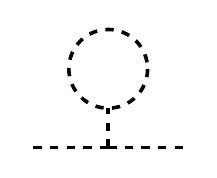
\begin{tikzpicture}[line width=1.3 pt, scale=1]
	\draw[scalarnoarrow] (0:1)--(0,0);
	% \node at (-140:1.2) {$e$};
	% \node at (140:1.2) {$e$};
	% \node at (.5,.3) {$\gamma$};	
	\draw[scalarnoarrow] (1.5,1) arc (360:0:.5);
%	\draw[scalarnoarrownoarrow] (2,0) arc (0:-180:.5);
	\draw[scalarnoarrow] (1,0) --(1,.5);
	\draw[scalarnoarrow] (1,0) --(2,0);
	% \node at (2.5,.3) {$\gamma$};	
\end{tikzpicture}
%} \\
Show that in the limit $m\to 0$ there is an IR divergence.
By thinking about the significance for the scalar potential of this part of the diagram
\vspace{1em}

\begin{tikzpicture}[line width=1.3 pt, scale=.5]
%	\draw[scalarnoarrow] (0:1)--(0,0);
	% \node at (-140:1.2) {$e$};
	% \node at (140:1.2) {$e$};
	% \node at (.5,.3) {$\gamma$};	
	\draw[scalarnoarrow] (1.5,1) arc (360:0:.5);
%	\draw[scalarnoarrownoarrow] (2,0) arc (0:-180:.5);
	\draw[scalarnoarrow] (1,0) --(1,.5);
%	\draw[scalarnoarrow] (1,0) --(2,0);
	% \node at (2.5,.3) {$\gamma$};	
\end{tikzpicture}
explain the meaning of this divergence.


\end{enumerate}


\item {\bf Bremsstrahlung.} [optional]
Show that the number of photons per decade of wavenumber 
produced by the sudden acceleration of a charge 
is (in the relativistic limit $-q^2 \gg m^2$) 
$$f_{IR}(q^2) = {\cor 2} { \alpha\over \pi} \ln \( { -q^2 \over m^2 } \) , $$
where $ q_\mu = p'_\mu -p_\mu$ is the change
of momentum and $m$ is the mass of the charge.  

\item {\bf Soft photons.}  [optional]

Check that the contribution from a single virtual photon (eq 2.60 of the lecture notes, with $n=2$) is 
\be {e^2 \over 2 } \int \dbar^4 d { - \ii \eta_{\rho \sigma} \over k^2 - m_\gamma^2 } 
\(  { p' \over p' \cdot k } 
- {p \over p \cdot k  } \)^\rho 
\(  { p^{'} \over - p' \cdot k } 
- {p \over - p \cdot k} \)^\sigma
= - { \alpha \over 2\pi } f_{IR} (q^2) \ln \( - q^2 \over m_\gamma^2 \) + \text{finite} \ee
where 
\be 
f_{IR}(q^2) = \int_0^1 dx  {  m_e^2 - q^2/2  \over m_e^2 - x (1-x) q^2 } - 1 .
\ee

[Hints: Wick rotate.  Scale out the overall magnitude of $k$, $k^\mu = k \hat k^\mu$.  Use Feynman parameters to combine $ (p \cdot \hat k) (p' \cdot \hat k)$.  ]
%Compare $f_{IR}(q_2)$ to the coefficient of the IR divergence $ \log \( E_c^2  \over m_\gamma^2 \)$ from the emission of one real soft photon.

Observe that this same integral appears in the cross section involving the emission of one real soft photon.  




\item {\bf Scale invariance in QFT in $D=0+0$, part 3.}  [I got this problem from Frederik Denef.]

We continue our study of QFT in $D=0+0$ with two fields:
$$ Z = \int dP_X dP_Y dX dY e^{ - H/ T} .$$
Let's start by considering again
\be \label{eq:3.3} H = \half P_X^2 + \half P_Y^2 + V(X,Y),~~~~V(X,Y) = aX^4 + b Y^8 \ee
for some nonzero constants $a,b$.   

A generic relevant deformation of \eqref{eq:3.3} will flow to a Gaussian fixed point $V(X,Y) \sim X^2 + Y^2$ in the IR.  
Some other, more fine-tuned deformations will flow to other fixed points.  
For example, $\delta V(X,Y) = \eps Y^4$ will flow to 
$V(X,Y) = X^4 + Y^4$.  But something more interesting happens for $\delta V(X,Y) = \eps X^2 Y^2$.  
This deformation is a relevant perturbation of \eqref{eq:3.3} in the sense that $\delta V(\lambda^{1/4} X, \lambda^{1/8} Y) = \lambda^\kappa V(X,Y)$ 
with $\kappa = 3/4 < 1$.  But it is not true that the model simply flows to a fixed point with $V \propto X^2 Y^2 $ in the IR.  
That's because the model with such a potential has a divergent partition function: 
$ \int_{-\infty}^\infty dX \int_{-\infty}^\infty dY e^{ - \eps X^2 Y^2 /T} \propto \sqrt{T\over \eps} \int { dX \over |X|} = \infty $.  We cannot throw away the higher-order terms 
because they regulate the large-$X$ and large-$Y$ behavior of the integral.  Thus, in this model, the UV does not completely decouple from the IR.
As a consequence, naive scaling arguments break down, and the partition function develops ``anomalous" logarithmic dependence on $T$ for small $T$.  


\begin{enumerate}
\item \label{part-n} Compute the partition function for the model \eqref{eq:3.3} deformed by $\delta V(X,Y) = \eps X^2 Y^2 $ analytically using Mathematica 
or some other symbolic software.  This will give a horrible mess of hypergeometric functions.  Expand it at small $T$ and you should find something of the form
\be\label{eq:power-law} Z = Z_0 T^c \log { \Lambda \over T} \ee
up to corrections suppressed by positive powers of $\sqrt{T/\Lambda}$.
Find the constants $Z_0, c, \Lambda$.  
The over all normalization $Z_0$ does not mean anything in classical statistical mechanics.  


%\answer{I'm going to wait to post this solution until next week.
%\end{enumerate}\end{enumerate}\end{document}
%}





\item Using \eqref{eq:power-law}, compute the dimensionless quantities $U/T$ and $C$.  (Without the logarithmic dependence on $T$, these would be equal.)  Check that in the strict limit $T\to 0$, you get the values for $U/T$ and $C$ that you would have guessed based on naive scaling arguments for $V \propto X^2 Y^2$.  Note that a logarithm varies more slowly than the $T^{1/2}$ corrections that we threw away. 

\item To what extent does the IR physics depend on the UV completion of the $V\propto X^2 Y^2 $ model?  We could have started with $ V = a X^8 + b Y^8+ \eps X^2 Y^2 $ instead.  This model would have different high-temperature physics.  Redo part \label{part-n} for this potential. 
You'll find an equally-horrendous, but different combination of hypergeometric functions.  Which of the parameters $Z_0, c, \Lambda$ are the same? 



\item The result of the previous part remains true for any other UV completion of the $V \propto X^2 Y^2$ model, as long as $\delta V = \eps X^2 Y^2$ 
remains a relevant deformation.  In fact, we could equally well just take $ V = \eps X^2 Y^2$ and impose a hard cutoff on the $X$ and $Y$ integrals at some fixed values $|X| \leq X_0, |Y|\leq Y_0$ (this is like $V = X^n + Y^n$ with $n \to \infty$).  Check that this again reduces to \eqref{eq:power-law}.  


\item \label{parte} In view of this apparent universality of \eqref{eq:power-law} at low $T$, it is desirable to have a way of deriving it without having to take the detour involving the horrendous hypergeometric functions.  Here is one way.  We use the hard cutoff $|X|\leq  L, |Y|\leq L$, so that the position-space factor is
\be\label{eq:cutoffZ} Z_V(T, L) = \int_{-L}^L dX \int_{-L}^L dY e^{ - X^2 Y^2 /T } \ee
where we've set $\eps = 1$ by a choice of temperature units.  
A rescaling of the integration variables $(X,Y) \to (T^{1/4} X, T^{1/4} Y) $ shows that $Z_V(T,L) = \sqrt{T} F(T^{-1/4} L) $ for some function $F$ of one variable.  To find $F$, compute $L \partial_L Z_V$ directly from \eqref{eq:cutoffZ}.  
By another suitable rescaling, show that $L\partial_L Z$ is finite and easily computable for $L^4 /T \to \infty$.  
Infer from this the dependence on the cutoff $L$ in the regime $T \ll L^4$ and thus the function $F$ in this regime.  This reproduces \eqref{eq:power-law}.  

\item We conclude that even when some kind of UV completion is required to give finite answers, the observable low-energy physics remains essentially independent of the UV completion.  The infinite number of possible UV completions all flow in the IR to a partition function of the same form \eqref{eq:power-law}, with the details of the UV completion all lumped into a single scale parameter $\Lambda$.  
In fact, in the absence of other reference scales that can be used to fix a unit of temperature, the parameter $\Lambda$ does not really label physically distinct models, since we can always choose units with $\Lambda=1$.  Equivalently, only dimensionless quantities (and relations between them) are physically meaningful.  Examples of such dimensionless quantities are $C$ and $u \equiv U/T$.  Show that $C$ and $u$ obey a universal relation $C = f(u)$ with $f(u)$ independent of $T$ and $\Lambda$, and thus independent of the UV completion of the $X^2Y^2 $ model.  In the same spirit, show that the function $g(u)$ in the flow equation $T\partial_T u = g(u) $ is independent of the UV completion.


\item Show that on the other hand $f(u)$ and $g(u)$ {\it do} depend on the IR part of the potential, for example by comparing the IR potential $V = X^2Y^2$ considered above to another IR potential such as $V = X^6 Y^6$.  

\end{enumerate}

\end{enumerate}




%\end{enumerate}
\end{document}
